\chapter{Séries de Fourier - Analyse fréquentielle des signaux périodiques}
\label{chap:series}
	Ce chapitre, ainsi que le suivant, s'intéresse à un outil fondamental de l'analyse des signaux : l'analyse fréquentielle ou spectrale. Elle vise à étudier un signal (temporel par exemple) dans un domaine dit dual : le domaine fréquentiel. En d'autres termes, cette analyse suppose que le signal peut être décomposé en une somme de fonctions périodiques, en l'occurrence (co)sinusoïdales. L'analyse fréquentielle consiste à analyser l'évolution de l'amplitude et la phase de ces termes en fonction de leur fréquence. Cette décomposition offre un autre "éclairage" du signal permettant de déceler des caractéristiques qui passent inaperçues dans le domaine temporel. La base de cette décomposition est appelée développement en série de Fourier. Cependant, il ne s'applique qu'aux fonctions périodiques. Dans le chapitre suivant, nous verrons que le développement en série de Fourier peut être modifié pour s'étendre à toutes les autres fonctions : on parlera alors de transformée de Fourier
	Le but de ces deux chapitres est de présenter les fondements théoriques de ces outils, leurs propriétés ainsi que leur mise en œuvre. L'analyse fréquentielle s'applique à toutes les fonctions, tous les signaux, réels ou complexes. Nous ne intéresserons ici qu'aux signaux à valeurs réels formant la majorité des cas d'étude en pratique.
	
	\section{Fonctions périodiques}
	On appelle une fonction périodique, de période $T_{0}$, se répète toutes les $T_{0}$ secondes. Cette période de répétition est appelée période fondamentale. L'inverse $F_{0}$, donnée par \ref{freq_fondamentale}, est appelée la fréquence fondamentale.
	
	\begin{equation}\label{freq_fondamentale}
	F_{0}=\frac{1}{T_{0}}
	\end{equation}
	
	Une fonction périodique f(t) vérifie donc la propriété suivante :
	\begin{equation}\label{Fonction_periodique}
	f(t)=f(t+kT_{0})~,~~\forall k\in \mathbb{Z}
	\end{equation}
	
	Cette fonction est nécessairement non bornée dans le temps. Seule la connaissance de la fonction pendant un intervalle est donc suffisant. Dans la suite, on se bornera à l'intervalle de temps $[0;T_{0}]$, voire $[-\frac{T_{0}}{2};+\frac{T_{0}}{2}]$.
	
	Parmi les fonctions périodiques, une famille particulière va nous intéresser : la famille des fonctions trigonométriques, intégrant les fonctions cosinusoïdales et sinusoïdales. Elles ont une propriété intéressante vis-à-vis de l'intégration. Dès qu'on intègre une fonction (co)sinusoïdale sur un intervalle de temps égal à la période fondamentale, alors celle-ci s'annule. De plus, si on considère des fonctions (co)sinusoïdales de fréquences multiples de la fréquence fondamentale et si on les intègre sur une période fondamentale, le résultat est encore une fois nul.
	\begin{equation}\label{key}
	\int_{T_{0}}cos(2\pi kF_{0}t)dt=\int_{T_{0}}sin(2\pi kF_{0}t)dt=0
	\end{equation}
	
	
	\section{Développement d'une fonction périodique sous la forme d'une série}
	
	\subsection{Principe}
	On peut montrer que toute fonction périodique x(t), de période $T_{0}$ peut être exprimée sous la forme d'une somme infinie ou série de termes $\Phi(k)$, comme le montre l'équation \ref{Decomposition_serie}, à condition que :
	\begin{itemize}
		\item ces termes forment un base de fonctions orthogonales
		\item elles sont des fonctions périodiques
	\end{itemize} 

	\begin{equation}\label{Decomposition_serie}
	x(t)=C_{0}\Phi_{0}(t)+C_{1}\Phi_{1}(t)+C_{2}\Phi_{2}(t)+...=\sum_{k=0}^{+\infty}C_{k}\Phi_{k}(t)
	\end{equation}

	
	Si les termes $\Phi_{k}$ peuvent être déterminés, on dit alors que la fonction peut être décomposée sous la forme d'une série de fonctions $\Phi_{k}$, liés avec x(t) par une série de coefficients $C_{k}$ qui sont les seuls inconnus à déterminer. k est appelé l'ordre de la fonction $\Phi_{k}$. L'orthogonalité est liée à l'opération de produit scalaire, définie par l'équation \ref{Produit_scalaire}, où T est la période commune à tous les termes $\Phi_{k}$. Si les fonctions sont complexes, le produit scalaire est donné par \ref{Produit_scalaire_complexe}, où le conjugué d'une des deux fonctions est requis.
	\begin{equation}\label{Produit_scalaire}
	\int_{T}\Phi_{m}(t)\Phi_{n}(t)dt
	\end{equation}
	\begin{equation}\label{Produit_scalaire_complexe}
	\int_{T}\Phi_{m}(t)\Phi_{n}^{*}(t)dt
	\end{equation}
	
	 Deux termes sont orthogonaux si leur produit scalaire est nul. Ainsi, la base de fonctions $\Phi_{k}$ forme une base orthogonale si les deux propriétés suivantes sont rencontrées :
	
	\begin{equation}\label{Def_base_fonctions_orthogonales}
	\int_{T}\Phi_{m}(t)\Phi_{n}(t)dt=\left \{
	\begin{array}{l l}
	K   & si~m=n \\
	0   & sinon \\
	\end{array}
	\right .
	\end{equation}
	
	Cette propriété se comprend aisément car elle permet de définir une relation permettant de calculer les coefficients $C_{k}$. En effet, si on réalise le produit scalaire entre x(t) et n'importe quelle fonction de la base $\Phi_{k}$, on isole le coefficient $C_{k}$, dont on peut calculer la valeur à l'aide de l'équation \ref{calcul_coef_decompo_serie}. Dans le cas où les fonctions $\Phi_{k}$ sont complexes, il faudra considérer son conjugué.
	\begin{equation*}
	\int_{T}x(t)\Phi_{k}(t)dt=C_{0}\int_{T}\Phi_{0}(t)\Phi_{k}(t)dt+C_{1}\int_{T}\Phi_{1}(t)\Phi_{k}(t)dt+...+C_{k}\int_{T}\Phi_{k}(t)\Phi_{k}(t)dt+...=0+0+...+C_{k}K+0...
	\end{equation*}
	\begin{equation*}
	\int_{T}x(t)\Phi_{k}(t)dt=C_{k}K
	\end{equation*}
	\begin{equation}\label{calcul_coef_decompo_serie}
	C_{k}=\frac{1}{K}\int_{T}x(t)\Phi_{k}(t)dt
	\end{equation}
	
	Cette décomposition en termes simples présente aussi un intérêt pour l'étude des systèmes linéaires. D'après le théorème de superposition, la réponse d'un système à une excitation x(t) se développant en une série de fonctions périodique $\Phi_{k}(t)$ peut être déterminée en additionnant les réponses individuelles aux fonctions $\Phi_{k}(t)$. Pour faciliter l'étude des systèmes linéaires, comme nous l'avons vu au chapitre 2, il est préférable de choisir des fonctions dont la forme générale n'est pas modifiée par l'effet du système linéaire, comme les fonctions de la famille exponentielle complexe.  

	
	
	\subsection{Série de fonctions trigonométriques}
	Les fonctions de la famille exponentielle complexe, qui s'écrivent $f(t)=Ae^{\sigma t}e^{j\omega t}$ ne sont pas périodiques sauf si $\sigma=0$. Dans ce cas, la fonction s'écrit : $f(t)=Acos(\omega t)+jAsin(\omega t)$ et représente une fonction trigonométrique complexe. En notant $T_{0}$ la période commune de tous les termes, la famille de fonctions $e^{jk\omega_{0} t}$, avec $\omega_{0}=\frac{2\pi}{T_{0}}$ et $k \in \mathbb{Z}$, forme une base de fonctions orthogonales. En effet, en posant $\Phi_{k}(t) = e^{jk\omega_{0}t}$, on peut montrer que : 
	\begin{equation*}
	\int_{0}^{T_{0}}\Phi_{m}(t)\Phi_{n}^{*}(t)dt=\int_{0}^{T_{0}}e^{jm\omega_{0}t}e^{-jn\omega_{0}t}dt=\int_{0}^{T_{0}}e^{j(m-n)\omega_{0}t}dt
	\end{equation*}
	\begin{itemize}
		\item si $m = n$, le produit scalaire est égal à : $\int_{0}^{T_{0}}\Phi_{n}(t)\Phi_{n}^{*}(t)dt=\int_{0}^{T_{0}}1dt=T_{0}$.
		\item si $m \neq n$, le produit scalaire s'annule (le calcul revient à intégrer des fonctions (co)sinusoïdales) multiples de la fréquence fondamentale sur une période fondamentale) :
	\end{itemize}
	\begin{equation*}
	\int_{0}^{T_{0}}e^{j(m-n)\omega_{0}t}dt=\int_{0}^{T_{0}}cos((m-n)\omega_{0}t)dt+j\int_{0}^{T_{0}}sin((m-n)\omega_{0}t)dt=0
	\end{equation*}
	
	En reprenant les équations \ref{Decomposition_serie} et \ref{calcul_coef_decompo_serie}, on en déduit que la fonction pourra se développer sous la forme de la série de fonctions exponentielles complexes suivantes :
	\begin{equation}\label{Dvpt_coef_Fourier_complexe}
	x(t)=\sum_{k=-\infty}^{+\infty}C_{k}e^{jk\omega_{0}t}
	\end{equation}
	
	où les coefficients $C_{k} \in \mathbb{C}$ seront calculés par :
	
	\begin{equation}\label{Calcul_coef_Fourier_complexe}
	C_{k}=\frac{1}{T_{0}}\int_{T_{0}}x(t)e^{-jk\omega_{0}t}dt~,~~\forall k \in \mathbb{Z}
	\end{equation}
	 

	Il aurait été possible de faire le même développement en faisant apparaitre coefficients réels. En repartant de l'équation \ref{Calcul_coef_Fourier_complexe}, on peut exprimer le coefficient complexe $C_{k}$ en fonction de deux coefficients réels, que nous notons $A_{k}^{'}$ et $B_{k}^{'}$.
	\begin{equation*}
	C_{k}=\frac{1}{T_{0}}\int_{T_{0}}x(t)(cos(k\omega_{0}t)-jsin(k\omega_{0}t))dt
	\end{equation*}
	\begin{equation*}
	C_{k}=\frac{1}{T_{0}}\int_{T_{0}}x(t)cos(k\omega_{0}t)dt-j\frac{1}{T_{0}}\int_{T_{0}}x(t)sin(k\omega_{0}t)dt
	\end{equation*}
	\begin{equation*}
	C_{k}=A_{k}^{'}-jB_{k}^{'}~,~~\forall k \in \mathbb{Z}
	\end{equation*}
	\begin{equation*}
	avec~~\left \{
	\begin{array}{l}
	A_{k}^{'}=\frac{1}{T_{0}}\int_{T_{0}}x(t)cos(k\omega_{0}t)dt\\
	B_{k}^{'}=\frac{1}{T_{0}}\int_{T_{0}}x(t)sin(k\omega_{0}t)dt \\
	\end{array}
	\right .
	\end{equation*}
	
	On remarque que le coefficient  $B_{k}^{'}=0$ pour k = 0. De plus, on observe des symétries entre les coefficients pour les valeurs positives et négatives de k : $A_{k}^{'}=A_{-k}^{'}$ et $B_{k}^{'}=-B_{-k}^{'}$.
	A partir de ces coefficients réels, on peut déterminer une nouvelle décomposition de la fonction x(t) en reprenant l'équation \ref{Dvpt_coef_Fourier_complexe}.
	\begin{equation*}
	x(t)=\sum_{k=-\infty}^{+\infty}C_{k}e^{jk\omega_{0}t}=\sum_{k=-\infty}^{+\infty}(A_{k}^{'}-jB_{k}^{'})e^{jk\omega_{0}t}
	\end{equation*}
	\begin{equation*}
	x(t)=(A_{0}^{'}-jB_{0}^{'})+\sum_{k=-\infty}^{-1}(A_{k}^{'}-jB_{k}^{'})e^{jk\omega_{0}t}+\sum_{k=1}^{+\infty}(A_{k}^{'}-jB_{k}^{'})e^{jk\omega_{0}t}
	\end{equation*}
	En utilisant les propriétés de symétries des coefficients, on peut exprimer la décomposition précédente en n'utilisant que des valeurs positives ou nulles pour k. En factorisant les coefficients, les termes exponentielles complexes peuvent être regroupés afin de faire apparaître des fonctions cosinus et sinus, donnant l'équation \ref{Dvpt_coef_Fourier_trigo}. 
	\begin{equation*}
	x(t)=A_{0}^{'}+\sum_{k=1}^{+\infty}(A_{k}^{'}-jB_{k}^{'})e^{jk\omega_{0}t}+\sum_{k=1}^{+\infty}(A_{k}^{'}-jB_{k}^{'})e^{jk\omega_{0}t}
	\end{equation*}
	\begin{equation*}
	x(t)=A_{0}^{'}+2\sum_{k=1}^{+\infty}A_{k}^{'}\frac{e^{jk\omega_{0}t}+e^{-jk\omega_{0}t}}{2}+2\sum_{k=1}^{+\infty}B_{k}^{'}\frac{e^{jk\omega_{0}t}-e^{-jk\omega_{0}t}}{2j}
	\end{equation*}
	\begin{equation*}
	x(t)=A_{0}^{'}+2\sum_{k=1}^{+\infty}A_{k}^{'}cos(k\omega_{0}t)+2\sum_{k=1}^{+\infty}B_{k}^{'}sin(k\omega_{0}t)
	\end{equation*}
	\begin{equation}\label{Dvpt_coef_Fourier_trigo}
	x(t)=A_{0}+\sum_{k=1}^{+\infty}A_{k}cos(k\omega_{0}t)+\sum_{k=1}^{+\infty}B_{k}sin(k\omega_{0}t)
	\end{equation}
	Le développement de la fonction x(t) se fait avec des fonctions trigonométriques $\Phi_{k}^{(1)}(t)=cos(k\omega_{0}t)$ et $\Phi_{k}^{(2)}(t)=sin(k\omega_{0}t)$, avec $k \in \mathbb{N}^{+}$ et des coefficients réels $A_{k}$ et $B_{k}$ donnés par \ref{Calcul_coef_Fourier_trigo_1} à \ref{Calcul_coef_Fourier_trigo_3}. 
	\begin{equation}\label{Calcul_coef_Fourier_trigo_1}
	A_{0}=A_{0}^{'}=C_{0}=\frac{1}{T_{0}}\int_{T_{0}}x(t)dt
	\end{equation}
	\begin{equation}\label{Calcul_coef_Fourier_trigo_2}
	A_{k}=2A_{k}^{'}=\frac{2}{T_{0}}\int_{T_{0}}x(t)cos(k\omega_{0}t)dt=2Re[C_{k}]~,~~~k \in \mathbb{N}^{+}
	\end{equation}
	\begin{equation}\label{Calcul_coef_Fourier_trigo_3}
	B_{k}=2B_{k}^{'}=\frac{2}{T_{0}}\int_{T_{0}}x(t)sin(k\omega_{0}t)dt=-2Im[C_{k}]~,~~~k \in \mathbb{N}^{+}
	\end{equation}
	On peut vérifier que la famille de fonctions composées de $\Phi_{k}^{(1)}(t)$ et $\Phi_{k}^{(2)}(t)$ forme une base de fonctions orthogonales, avec :
	\begin{equation}\label{}
	\int_{T}\Phi_{m}^{(k)}(t)\Phi_{n}^{(l)}(t)dt=\left \{
	\begin{array}{l l}
	\frac{T_{0}}{2}   & si~m=n~et~si~k=l \\
	0   & sinon \\
	\end{array}
	\right .
	\end{equation}
	
	
	

	
	On peut donc décomposer toute les fonctions périodiques x(t) de période $T_{0}$ sous la forme d'une série de fonctions trigonométriques, de périodes  $\frac{T_{0}}{k}$. Ce développement est appelé développement en série de Fourier, qui consiste à déterminer des coefficients appelés coefficients de Fourier. Il existe sous différentes formes, que nous allons récapituler dans la prochaine partie.

	
	
	\section{Calcul des coefficients d'une série de Fourier}	
	
	Nous passons en revue les différentes formes de décomposition en série de Fourier d'une fonction, que l'on suppose à valeurs réels.
	
	\subsection{Forme trigonométrique}
	Elle constitue une forme très courante de développement en série de Fourier. Elle est basée sur une décomposition en fonction cosinus et sinus, comme nous l'avons montré avec \ref{Dvpt_coef_Fourier_trigo}. Le développement d'une fonction périodique x(t), de période $T_{0}$ en série de Fourier sous la forme trigonométrique s'écrit :
	\begin{equation}\label{Serie_Fourier_Trigo}
	x(t)=A_{0}+\sum_{k=1}^{+\infty}A_{k}cos(k\omega_{0}t)+\sum_{k=1}^{+\infty}B_{k}sin(k\omega_{0}t)~,~~k \in \mathbb{N^{+}}
	\end{equation}
	
	avec les expressions suivantes pour les coefficients :
	\begin{equation}\label{Coef_Serie_Fourier_trigo_1}
	A_{0}=\frac{1}{T_{0}}\int_{T_{0}}x(t)dt
	\end{equation}
	\begin{equation}\label{Coef_Serie_Fourier_trigo_2}
	A_{k}=\frac{2}{T_{0}}\int_{T_{0}}x(t)cos(k\omega_{0}t)dt~,~~~k \in \mathbb{N}^{+}
	\end{equation}
	\begin{equation}\label{Coef_Serie_Fourier_trigo_3}
	B_{k}=\frac{2}{T_{0}}\int_{T_{0}}x(t)sin(k\omega_{0}t)dt~,~~~k \in \mathbb{N}^{+}
	\end{equation}
	
	On remarque que le terme $A_{0}$ représente la valeur moyenne ou composante continue de la fonction x(t). Le développement en série de Fourier est donc la superposition de la valeur moyenne et de fonctions cosinusoïdaux et sinusoïdaux de fréquences positives et multiples de la fréquence fondamentale. \\
	
	\underline{\textbf{Remarque : bornes de l'intégration pour le calcul des coefficients de Fourier :}}
	
	Comme le montre les équations \ref{Coef_Serie_Fourier_trigo_1} à \ref{Coef_Serie_Fourier_trigo_3}, le calcul se fait par une intégration du produit entre la fonction à développer et une fonction trigonométrique, sur une période fondamentale. Une question légitime est : où doit-on commencer l'intégration ? La réponse est peu importe. La fonction étant périodique et non bornée dans le temps, on peut faire démarrer une période n'importe où. On peut aussi bien fixer les bornes d'intégration entre 0 et $T_0$, qu'entre $-\frac{T_0}{2}$ et $+\frac{T_0}{2}$, le résultat du calcul des coefficients de Fourier restera le même. Le choix des bornes de l'intégration sera uniquement guidé par une simplification du calcul.\\ 
	
	
	
	\underline{\textbf{Exemple : Développement en série de Fourier d'un signal carré\\}}
	
	On se propose de développer en série de Fourier, sous leur forme trigonométrique, la fonction x(t) décrite par la figure ci-dessous et représentant un signal carré de période $T_{0}$ définie sur une période fondamentale par :
	\begin{equation*}
	x(t)=\left \{
	\begin{array}{l l}
	+A   & si~t \in [0;\frac{T_{0}}{2}] \\
	-A   & si~t \in [\frac{T_{0}}{2};T_{0}] \\
	\end{array}
	\right .
	\end{equation*}
	
	\begin{figure}[h!]
		\centering
		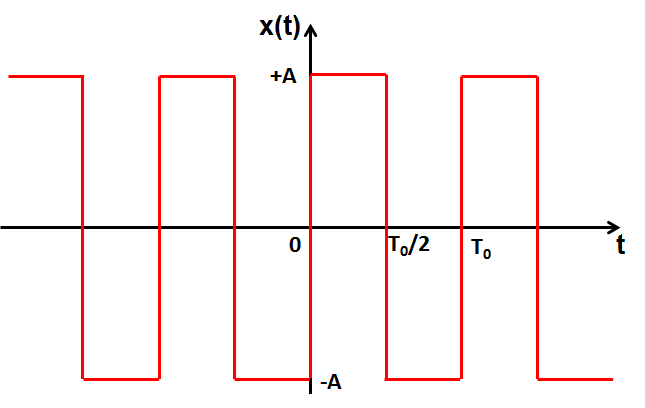
\includegraphics[scale=0.5]{images/signal_carre.png}
		\caption{Signal carré de période $T_{0}$}	
		\label{Fig:Signal_Carre} 
	\end{figure}
	
	On remarque que le signal a une valeur moyenne nulle donc la composante $A_{0}=0$, ce que confirme le calcul de ce coefficient de Fourier : $A_{0}=\frac{1}{T_{0}}\int_{0}^{T_{0}}x(t)dt=\frac{1}{T_{0}}(\int_{0}^{\frac{T_{0}}{2}}Adt+\int_{\frac{T_{0}}{2}}^{T_{0}}-Adt)=0$. Les coefficients de Fourier liés aux termes cosinusoïdaux se calcule à l'aide de \ref{Coef_Serie_Fourier_trigo_2}. La fonction sinus s'annulant pour tous les multiples entiers de $\pi$, les coefficients $A_{k}$ sont tous nuls.
	\begin{equation*}
	A_{k}=\frac{2}{T_{0}}\int_{T_{0}}x(t)cos(k\omega_{0}t)dt=\frac{2}{T_{0}}(\int_{0}^{\frac{T_{0}}{2}}Acos(k\omega_{0}t)dt+\int_{\frac{T_{0}}{2}}^{T_{0}}-Acos(k\omega_{0}t)dt)
	\end{equation*}
	\begin{equation*}
	A_{k}=\frac{2A}{k\omega_{0}T_{0}}([sin(k\omega_{0}t)]_{0}^{\frac{T_{0}}{2}}-[sin(k\omega_{0}t)]_{\frac{T_{0}}{2}}^{T_{0}})=\frac{A}{k\pi}(sin(k\pi)-0-sin(k2\pi)+sin(k\pi))
	\end{equation*}
	\begin{equation*}
	A_{k}=\frac{2A}{k\pi}sin(k\pi)=0~~\forall k \in \mathbb{N^{+}}
	\end{equation*}
	Les coefficients de Fourier liés aux termes sinusoïdaux se calcule à l'aide de \ref{Coef_Serie_Fourier_trigo_3}.
	\begin{equation*}
	B_{k}=\frac{2}{T_{0}}\int_{T_{0}}x(t)sin(k\omega_{0}t)dt=\frac{2}{T_{0}}(\int_{0}^{\frac{T_{0}}{2}}Asin(k\omega_{0}t)dt+\int_{\frac{T_{0}}{2}}^{T_{0}}-Asin(k\omega_{0}t)dt)
	\end{equation*}
	\begin{equation*}
	B_{k}=\frac{2A}{k\omega_{0}T_{0}}([-cos(k\omega_{0}t)]_{0}^{\frac{T_{0}}{2}}-[-cos(k\omega_{0}t)]_{\frac{T_{0}}{2}}^{T_{0}})=\frac{A}{k\pi}(cos(0)-cos(k\pi)-cos(k\pi)+cos(k2\pi))
	\end{equation*}
	\begin{equation*}
	B_{k}=\frac{2A}{k\pi}(1-cos(k\pi))~~\forall k \in \mathbb{N^{+}}
	\end{equation*}
	Selon la parité de l'ordre k, ce coefficient ne prend pas la même valeur :
	\begin{equation*}
	B_{k}=\left \{
	\begin{array}{l l}
	+0   & si~k~est~pair. \\
	\frac{4A}{k\pi}   & si~k~est~impair. \\
	\end{array}
	\right .
	\end{equation*}
	La fonction carrée x(t) peut donc se décomposer à l'aide de la série de Fourier suivante :
	\begin{equation*}
	x(t)=\frac{4A}{\pi}(sin(\omega_{0}t)+\frac{1}{3}sin(3\omega_{0}t)+\frac{1}{5}sin(5\omega_{0}t)+...)=\frac{4A}{\pi}\sum_{k=0}^{+\infty}\frac{1}{2k+1}sin((2k+1)\omega_{0}t)
	\end{equation*}
	
	
	
	On remarque que les coefficients de Fourier que l'on a déterminé sont indépendants de la valeur de la fréquence $f_{k}=\frac{k}{T_{0}}$, mais seulement de l'ordre du terme trigonométrique. Ainsi, quelle que soit sa fréquence fondamentale, un signal carré présentant la même forme d'onde que x(t) présentera la même décomposition en série de Fourier. Seule la pulsation fondamentale $\omega_{0}$ changera.
	
	
	\subsection{Forme polaire}
	
	La forme trigonométrique, faisant apparaitre des termes cosinusoïdaux et sinusoïdaux, peut être transformée pour ne faire apparaître que des termes cosinusoïdaux. En effet, on peut remarque la série de Fourier \ref{Serie_Fourier_Trigo} peut s'écrire :
	\begin{equation}\label{Serie_Fourier_Polaire}
	x(t)=A_{0}+\sum_{k=1}^{+\infty}A_{k}cos(k\omega_{0}t)+\sum_{k=1}^{+\infty}B_{k}sin(k\omega_{0}t)=A_{0}+\sum_{k=1}^{+\infty} \rho_{k}cos(k\omega_{0}t-\phi_{k})
	\end{equation}
	
	avec :
	\begin{equation}\label{Coef_Serie_Fourier_polaire}
	\left \{
	\begin{array}{l}
	\rho_{k}=\sqrt{A_{k}^{2}+B_{k}^{2}} \\
	\phi_{k}=-arctan(\frac{B_{k}}{A_{k}}) \\
	\end{array}
	\right . ~\Rightarrow~	\left \{
	\begin{array}{l}
	A_{k}=\rho_{k}cos\phi_{k} \\
	B_{k}=\rho_{k}sin\phi_{k} \\
	\end{array}
	\right .
	\end{equation}
	
	Les coefficients de Fourier définissent cette fois l'amplitude et la phase d'un terme cosinusoïdal. Ils constituent donc un vecteur de Fresnel ou phaseur, d'où la notion de forme polaire.\\
	
	\underline{\textbf{Exemple : Développement en série de Fourier d'un signal carré\\}}
	
	On reprend l'exemple précédent mais on cherche cette fois la représentation polaire des coefficients de Fourier. En repartant de la forme trigonométrique, on peut les déterminer :
	\begin{equation*}
	\rho_{k}=\sqrt{A_{k}^{2}+B_{k}^{2}}=B_{k}=\frac{4A}{k\pi}~,~k~entier~impaire
	\end{equation*}
	\begin{equation*}
	\phi_{k}=-arctan(\frac{B_{k}}{A_{k}})=-\frac{\pi}{2}
	\end{equation*}
	
	\subsection{Forme complexe}
	
	Il s'agit de la forme la plus compacte de développement en série de Fourier que l'on privilégie souvent en pratique. Elle est basée sur la décomposition en exponentielle complexe, comme nous l'avons montré avec \ref{Dvpt_coef_Fourier_complexe}. Le développement d'une fonction périodique x(t), de période $T_{0}$ en série de Fourier sous la forme complexe s'écrit :
	
	\begin{equation}\label{Serie_Fourier_Complexe}
	x(t)=\sum_{k=-\infty}^{+\infty}C_{k}e^{jk\omega_{0}t}
	\end{equation}
	
	avec les expressions pour les coefficients :
	
	\begin{equation}\label{Coef_Serie_Fourier_Complexe}
	C_{k}=\frac{1}{T_{0}}\int_{T_{0}}x(t)e^{-jk\omega_{0}t}dt~,~~\forall k \in \mathbb{Z}
	\end{equation}
	
	On remarque que le terme $C_{0}=\frac{1}{T_{0}}\int_{T_{0}}x(t)dt$ représente la valeur moyenne de x(t). On remarque aussi le lien entre cette forme et les formes trigonométriques et polaires :
	\begin{equation}\label{Lien_formes_coef_Fourier}
	2C_{k}=A_{|k|}-jB_{|k|}=\rho_{k}e^{j\phi_{k}}~~\forall k \in \mathbb{Z^{*}}
	\end{equation}
	
	Cependant, contrairement aux deux autres formes précédentes, les coefficients de Fourier sont définis pour des ordres positifs et négatifs. En d'autres termes, pour des fréquences positives et négatives. On peut vérifier une propriété de symétrie des coefficients complexes entre les fréquences positives et négatives : ils sont égaux en module, mais opposés en phase. En d'autres termes, les coefficients sont conjugués.\\
	\begin{equation}\label{key}
	C_k=C_{-k}^{*}~~\Rightarrow~|C_k|=|C_{-k}|~et~arg(C_k)=-arg(C_{-k})
	\end{equation}
	
	\underline{\textbf{Exemple : Développement en série de Fourier d'un signal carré\\}}
	
	On reprend l'exemple précédent mais on cherche cette fois la représentation complexe des coefficients de Fourier. En utilisant l'équation \ref{Coef_Serie_Fourier_Complexe}, on détermine :
	\begin{equation*}
	C_{k}=\frac{1}{T_{0}}\int_{0}^{T_{0}}x(t)e^{-jk\omega_{0}t}dt=\frac{1}{T_{0}}(\int_{0}^{\frac{T_{0}}{2}}Ae^{-jk\omega_{0}t}dt-\int_{\frac{T_{0}}{2}}^{T_{0}}Ae^{-jk\omega_{0}t}dt)
	\end{equation*} 
	\begin{equation*}
	C_{k}=\frac{A}{-jk\omega_{0}T_{0}}([e^{-jk\omega_{0}t}]_{0}^{\frac{T_{0}}{2}}-[e^{-jk\omega_{0}t}]_{\frac{T_{0}}{2}}^{T_{0}})=\frac{jA}{k2\pi}(e^{-jk_pi}-1-e^{-jk2\pi}+e^{-jk_pi})
	\end{equation*}
	\begin{equation*}
	\frac{jA}{k\pi}(e^{-jk\pi}-1)
	\end{equation*}
	Si k est pair, $e^{-jk\pi}=1~\Rightarrow~C_{k}=0$. Si k est impair,  $e^{-jk\pi}=-1~\Rightarrow~C_{k}=\frac{-2jA}{k\pi}$. En comparant les différentes formes des coefficients de Fourier, on vérifie bien l'équation \ref{Lien_formes_coef_Fourier}.
	
	
	\subsection{Somme partielle}
		
	Le développement en série de Fourier suppose la somme d'un nombre infini de termes trigonométriques ou exponentiels complexes. En pratique, si on cherche à calculer chacun des termes de la série de Fourier, on n'en calculera qu'un nombre fini N. On parle alors de somme partielle $S_{N}$, définie par :
	\begin{equation}\label{Somme_partielle}
	S_{n}=A_{0}+\sum_{k=1}^{N}A_{k}cos(k\omega_{0}t)+\sum_{k=1}^{N}B_{k}sin(k\omega_{0}t)=\sum_{k=-N}^{+N}C_{k}e^{jk\omega_{0}t}
	\end{equation}
	
	Dans les cas où la série de Fourier d'une fonction existe (nous discuterons de ce point dans la prochaine partie), alors la somme partielle converge vers la décomposition en série de Fourier au fur et à mesure qu'on augmente le nombre N de termes additionnés.
	L'exemple ci-dessous reprend le signal carré étudié précédemment pour illustrer la convergence de la somme partielle. On prend A = 1 et $T_{0} = 1 s$, d'où une fréquence fondamentale de 1 Hz. Le tableau ci-dessous donne les valeurs des coefficients de Fourier en fonction de l'ordre. Il montre clairement que plus l'ordre augmente, plus l'amplitude du terme décroit.
	
	\begin{table}[h!]
		\centering
		\begin{tabular}{|c|c|c|c|}
			\hline
			\textbf{Ordre n} & \textbf{$A_{n}$} & \textbf{$B_{n}$} & \textbf{$C_{n}$}\\
			\hline
			1 & 0 & $\frac{4}{\pi}$ & -j$\frac{2}{\pi}$ \\	
			\hline
			3 & 0 & $\frac{4}{3\pi}$ & -j$\frac{2}{3\pi}$ \\	
			\hline
			5 & 0 & $\frac{4}{5\pi}$ & -j$\frac{2}{5\pi}$ \\	
			\hline
			7 & 0 & $\frac{4}{7\pi}$ & -j$\frac{2}{7\pi}$ \\	
			\hline
			... & ... & ... & ... \\
			\hline
		\end{tabular}	
	\end{table}
	
	La figure \ref{Fig:somme_partielle} compare le signal carré et la somme partielle, pour différentes valeurs d'ordre de sommation N. Lorsque N est faible, on voit clairement l'effet de chacun des termes sinusoïdaux qui ajoute une oscillation de période $\frac{T_{0}}{k}$. Plus on augmente N, plus il est difficile de séparer leurs effets respectifs et la somme partielle reproduit de plus en plus fidèlement le signal carré. Cependant, même en augmentant fortement l'ordre N (par exemple, jusqu'à 99), on observe toujours des oscillations parasites notamment à proximité des transitions du signal. Ce phénomène s'appelle le phénomène de Gibbs. La somme partielle tronque la série de Fourier et supprime les termes sinusoïdaux de plus haute fréquence. Or, ce sont ceux-ci qui constituent les variations rapides d'une fonction. Dans un cas pratique, il est donc impossible de faire disparaître le phénomène de Gibbs. Au mieux, on peut le minimiser en augmentant très fortement l'ordre N. 
	
	 
	\begin{figure}[h!]
	 	\centering
	 	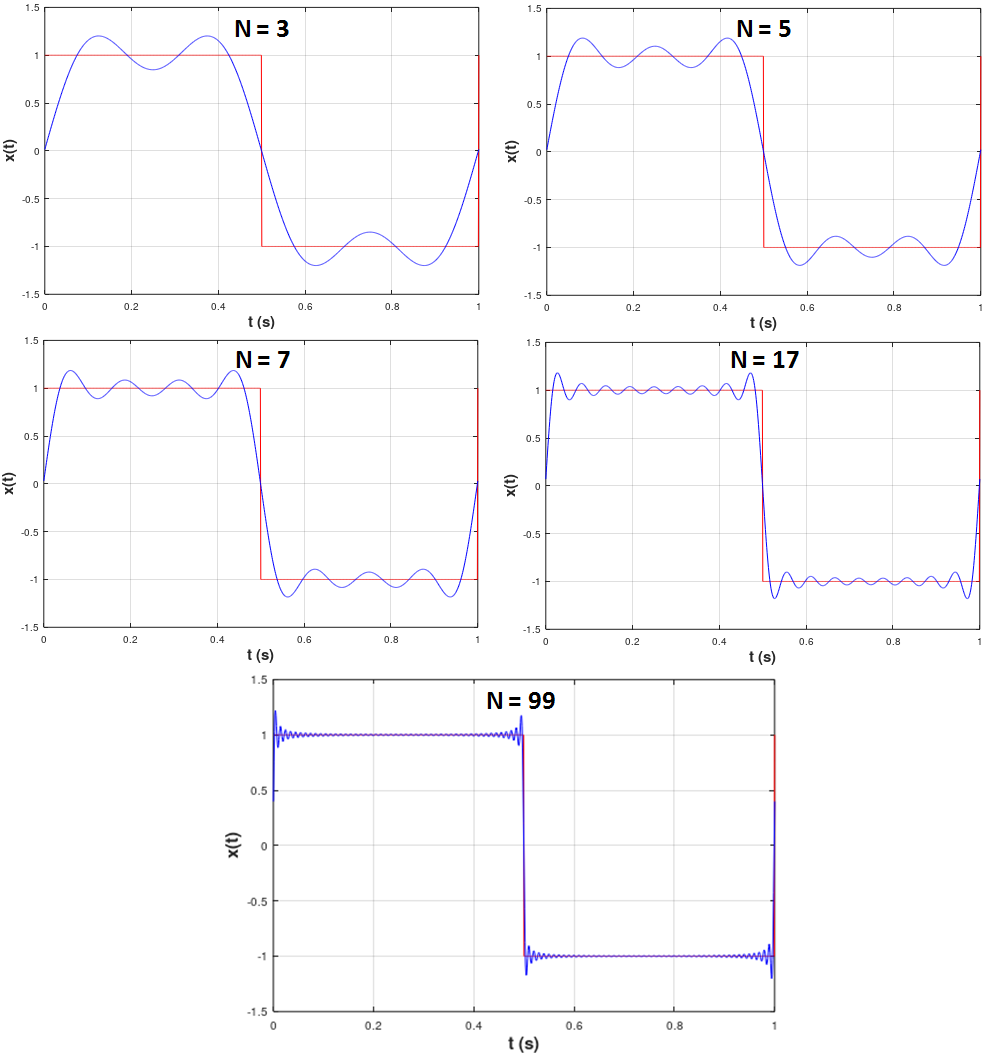
\includegraphics[scale=0.5]{images/convergence_somme_partielle.png}
	 	\caption{Convergence d'une somme partielle (signal carré) en fonction de l'ordre maximale}	
	 	\label{Fig:somme_partielle} 
	\end{figure}
	 

	
	
	\vspace{1\baselineskip}
	
	
	\section{Convergence des séries de Fourier - Théorème de Dirichlet}
	Avant de lister les propriétés des séries de Fourier, nous devons aborder une question fondamentale avant de réaliser le développement en série de Fourier : qu'est-ce qui nous garantit la série de Fourier va converger vers la fonction x(t) ? En effet, le calcul des coefficients repose sur celui de l'intégrale \ref{Coef_Serie_Fourier_Complexe}. Or, si cette intégrale diverge, alors la série de Fourier ne peut pas converger et le développement en série de Fourier devient impossible. Il est donc indispensable de déterminer les conditions qui garantissent cette convergence.
	
	Le but de cette partie n'est pas de démontrer rigoureusement ces conditions, mais simplement de les énoncer. Cette question sera traiter dans le cours d'Anayse et algèbre.\\
	
	
	Les conditions de convergence des séries de Fourier sont définies par le théorème de Dirichlet. Ces questions se posent naturellement dès que la fonction x(t) que l'on cherche à développer présente des discontinuités. Avant de l'énoncé, il est nécessaire de définir certains termes. 
	
	\subsection{Continuité par morceaux}
	
	Une fonction x(t) est dite continue par morceaux sur un intervalle I (par exemple $[0;T_{0}]$) si elle est continue sur I, sauf en un nombre fini de points qui sont des points de discontinuités de première espèce. En un point de discontinuité de première espèce apparaissant en $t_{i}$, la fonction a une limite à droite $x(t_{i}^{+})$ et une limite à gauche $x(t_{i}^{-})$.
	
	\subsection{Classe $C^{1}$}
	On dit qu'une fonction x(t) défini sur un intervalle I est de classe $C^{1}$ par morceaux sur I si elle est continue par morceaux sur I, mais aussi si elle est dérivable sur I sauf en un nombre fini de points, avec la dérivée x' continue par morceaux sur I.
	
	\subsection{Théorème de Dirichlet}
	Soit x une fonction périodique, de période $T_{0}$, de classe $C^{1}$ par morceaux
	alors la série de Fourier associée à x converge en tout point de discontinuité vers $\frac{x(t_{i}^{+})+x(t_{i}^{-})}{2}$. Dans le cas complexe, en ce point, la série de Fourier converge vers :
	\begin{equation}\label{key}
	\sum_{k=-\infty}^{+\infty}C_{k}e^{jk\omega_{0}t_{i}}=\frac{x(t_{i}^{+})+x(t_{i}^{-})}{2}
	\end{equation}
	Dans le cas d'une forme trigonométrique, elle converge vers :
	\begin{equation}\label{key}
	A_{0}+\sum_{k=1}^{+\infty}A_{k}cos(k\omega_{0}t_{i})+\sum_{k=1}^{+\infty}B_{k}sin(k\omega_{0}t_{i})=\frac{x(t_{i}^{+})+x(t_{i}^{-})}{2}
	\end{equation}
	
	Dans cette situation, la série de Fourier converge en tout point de l'intervalle I. On peut donc décomposer la fonction x(t) en une série de Fourier. Dans la majorité des cas pratiques, les signaux périodiques sont continus et dérivables sur toute leur période. Il respecte les conditions du théorème de Dirichlet et sont donc décomposables en série de Fourier.	\\
	
	
	\underline{\textbf{Exemple : signal périodique de forme exponentiel}}
	
	On considère une fonction périodique x, définie sur l'intervalle $[0;2\pi[$ par $x(t)=e^{t}$. Peut-on développer cette fonction en série de Fourier ?\\
	
	La fonction est continue sur tout l'intervalle, sauf en t = 0, puisque :
	\begin{equation*}
	\lim_{t \to 0^{-}}x(t)=e^{2\pi}~~~et~~~\lim_{t \to 0^{+}}x(t)=1
	\end{equation*}
	
	Il en est de même pour tous les points $t_{k}=k2\pi$, $k \in \mathbb{Z}$. La question de convergence de la série de Fourier se pose donc. Cependant, on vérifie que la fonction est continue par morceau sur l'intervalle fondamental, sauf en t=0. Mais cette discontinuité est de première espèce puisqu'elle admet une limite à droite et à gauche. Le même raisonnement s'applique à sa dérivée, donc il s'agit d'une fonction de classe $C^{1}$ par morceaux. Cela est vrai non seulement sur l'intervalle fondamental, mais aussi sur l'ensemble $\mathbb{R}$. Les hypothèses du théorème de Dirichlet
	sont satisfaites et on peut l'appliquer :
	\begin{itemize}
		\item si $t \neq 2k\pi~~\forall k \in \mathbb{Z}$, alors la série de Fourier en t converge vers x(t).
		\item si $ t = t_{k}= 2k\pi~~\forall k \in \mathbb{Z}$, alors la série de Fourier converge vers $\frac{x(t_{k}^{+})+x(t_{k}^{-})}{2}=\frac{1+e^{2\pi}}{2}$
	\end{itemize}

	On pourra vérifier que le développement en série de Fourier, sous forme complexe, de cette fonction donne :
	\begin{equation*}
	C_{k}=\frac{1}{2\pi(1-jk)}(e^{2\pi}e{-jk}-1)
	\end{equation*}
	
	\vspace{1\baselineskip}

	
	
	\section{Propriétés des séries de Fourier}
	Dans cette partie, nous passons en revue les propriétés des séries de Fourier. Certaines d'entre elles présentent un intérêt pratique certain car elles facilitent le calcul des coefficients de la série.
	
	\subsection{Linéarité}
	La décomposition en série de Fourier est une opération linéaire. Le principe de superposition s'applique donc. Soit deux fonctions périodiques x(t) et y(t) dont les développements en série de Fourier, dont les termes respectifs sont notés $\alpha_{k}$ et $\beta_{k}$. Soit la fonction $z(t)=ax(t)+by(t)$, avec a et b $\in \mathbb{R}$, alors la fonction z(t) est une fonction périodique qui peut aussi être développée en série de Fourier. Ces coefficients de Fourier sont $\gamma_{k}=a\cdot \alpha_{k}+b \cdot \beta_{k}$.
	
	\subsection{Changement de période}
	Soit une fonction x(t) possédant une forme donnée. Si sa fréquence fondamentale change, les coefficients de Fourier restent inchangés.
	
	\subsection{Théorème du retard}
	Lorsqu'une fonction temporelle est décalée (retardée ou avancée d'une durée $t_{0}$), l'amplitude de ses coefficients de Fourier n'est pas affectée. Seule la phase est modifiée (traduisant un décalage temporel de l'ensemble des termes trigonométriques). Soit la fonction x(t) dont les coefficients de Fourier complexes sont notés $\alpha_{k}$, et une fonction y(t) une version retardée d'une durée $t_{0}$, alors le développement en série de Fourier de la fonction y peut s'écrire :
	\begin{equation*}
	y(t)=x(t-t_0)=\sum_{k=-\infty}^{+\infty}\alpha_{k}^{jk\omega_{0}(t-t_0)}=\sum_{k=-\infty}^{+\infty}\alpha_{k}e^{-jk\omega_{0}t_0}e^{jk\omega_{0}t}
	\end{equation*}
	Les coefficients de Fourier complexes $\beta_{k}$ de la série représentant y(t) s'écrivent donc :
	\begin{equation}\label{Theoreme_retadr_serie_Fourier}
	\beta_{k}=\alpha_{k}e^{-jk\omega_{0}t_0}
	\end{equation}
	
	Un retard d'une durée $t_{0}$ se traduit donc comme une modification de phase égale à $e^{-jk\omega_{0}t_0}$ pour l'ensemble des termes de la série de Fourier.\\
	
	\underline{\textbf{Exemple : signal carré retardé}}
	On reprend l'exemple du signal carré précédemment étudié (figure \ref{Fig:Signal_Carre} ), mais on le retarde d'une demi période (on remarquera que cela est équivalent à une avance d'une demi période), comme le montre la figure ci-dessous. A partir des coefficients de Fourier $C_k$, $A_k$ et $B_k$ que nous avons déjà calculé pour le signal carré et du théorème du retard, nous pouvons aisément déduire ceux de cette version retardée. 
	\begin{figure}[h!]
		\centering
		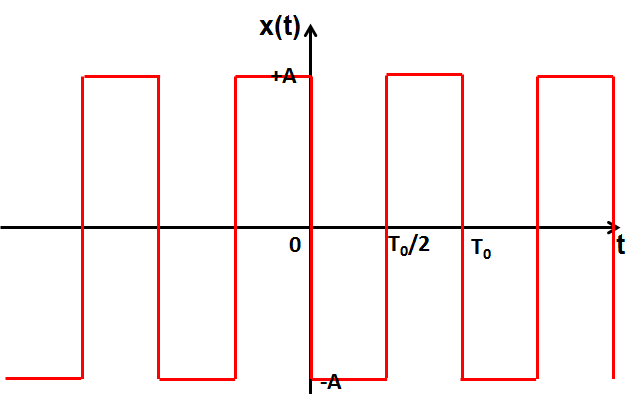
\includegraphics[scale=0.5]{images/signal_carre_retard.png}
	\end{figure}
	Les termes $C_0$ et $A_0$, représentant la valeur moyenne ne sont pas modifiés. Les coefficients complexes deviennent :
	\begin{equation*}
	C_k^{'}=C_ke^{-jk\omega_{0}\frac{T_0}{2}}=C_ke^{-jk_pi}=\frac{jA}{k\pi}(1-e^{-jk\pi})
	\end{equation*}
	Seuls les coefficients d'ordre k impair sont non nuls et sont égaux à $C_k^{'}=+\frac{2jA}{k\pi}$. Sous la forme trigonométrique, tous les coefficients $A_k^{'}$ restent nuls. Les coefficients $B_k^{'}$ sont non nuls pour les coefficients d'ordre k impair et égaux à $B_k^{'}=-\frac{4A}{k\pi}$.\\
	
	
	
	\subsection{Dérivée}
	Soit une fonction périodique x(t) présentant un développement en série de Fourier complexe, dont les coefficient sont notés $\alpha_{k}$. La fonction $y(t)=\frac{dx}{dt}$ est aussi périodique et peut être développée en série de Fourier. Ses coefficients de Fourier $\beta_{k}$ sont donnés par :
	\begin{equation}\label{derivee_Serie_Fourier}
	\beta_{k}=(jk\omega_{0})\alpha_{k}
	\end{equation}
	De même si $y(t)=\frac{d^{m}x}{dt^{m}}$, alors les coefficients de Fourier sont reliés par :
	\begin{equation}\label{derivee_Serie_Fourier_multiple}
	\beta_{k}=(jk\omega_{0})^{m}\alpha_{k}
	\end{equation}
	
	\subsection{Intégration}
	On retrouve la propriété inverse de la propriété de dérivée. Si la fonction $y(t)=\int x(\tau)d\tau$, alors les coefficients de Fourier sont reliés par :
	\begin{equation}\label{integrale_Serie_Fourier}
	\beta_{k}=\frac{\alpha_{k}}{jk\omega_{0}}
	\end{equation}
	De même si la fonction y est une intégrale multiple d'ordre m de la fonctio x,  alors les coefficients de Fourier sont reliés par :
	\begin{equation}\label{integrale_Serie_Fourier_multiple}
	\beta_{k}=\frac{\alpha_{k}}{(jk\omega_{0})^{m}}
	\end{equation}
	
	\underline{\textbf{Exemple : signal triangulaire}}
	On considère la fonction y de période $T_{0}$ décrit à la figure ci-dessous. Développez en série de Fourier cette fonction. 
	
	\begin{figure}[h!]
		\centering
		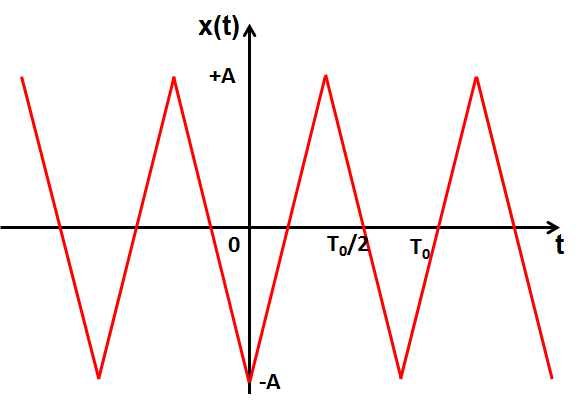
\includegraphics[scale=0.5]{images/signal_triangulaire.png}	
	\end{figure}
	
	On peut utiliser les équations \ref{Coef_Serie_Fourier_Complexe} ou \ref{Coef_Serie_Fourier_trigo_1} pour déterminer l'expression théorique des coefficients de Fourier. Néanmoins, le calcul de l'intégrale va passer par une intégration par partie. Etant donné que nous avons déjà développé en série de Fourier le signal carré x(t) et en remarquant que $y(t)=\frac{4}{T_0}\int x(\tau)d\tau$, on peut facilement déterminer le développement en série de Fourier de la fonction y en appliquant la propriété d'intégration.  \\
	Soit $\alpha_{k}=\frac{jA}{k\pi}(e^{-jk\pi}-1)$ les coefficients de Fourier associés à x(t), ceux de y(t), notés $\beta_{k}$ seront donnés par :
	\begin{equation*}
	\beta_{k} = \frac{4}{T_0}\alpha_{k}\frac{1}{jk\omega_{0}}=\frac{2\alpha_{k}}{jk\pi}
	\end{equation*}
	\begin{equation*}
	\beta_{k} =\frac{2A}{(k\pi)^{2}}(e^{-jk\pi}-1)
	\end{equation*}
	
	On trouve que $\beta_{k} = 0$ si k est pair et $\beta_k=\frac{4A}{(k\pi)^{2}}$ si k est impair. En forme trigonométrique, ce coefficient s'écrira : $A_{k} = \frac{-8A}{(k\pi)^{2}}$ et $B_k = 0$. Le développement en série de Fourier de la fonction y(t) s'écrit donc :
	\begin{equation*}
	y(t)=\frac{-8A}{\pi^{2}}\sum_{k=1}^{+\infty}\frac{1}{(2k+1)^{2}}cos((2k+1)\omega_{0}t)
	\end{equation*}
	
	\subsection{Egalités entre coefficients de Fourier}
	Les coefficients de Fourier, selon la forme employée pour la décomposition de Fourier, sont reliés par les équations suivantes :
	\begin{equation}\label{key}
	C_0=A_0~~~~~C_k=\frac{A_k-jB_k}{2}~\forall~k \in \mathbb{N^{+}}~~~~~C_{-k}=\frac{A_k+jB_k}{2}~\forall~k \in \mathbb{N^{+}}
	\end{equation}
	\begin{equation}\label{key}
	A_k=C_k+C_{-k}~~~~~B_k=C_k-C_{-k}~\forall~k \in \mathbb{N^{+}}
	\end{equation}
	
	\subsection{Symétries temporelles}
	
	Le signal temporel peut présenter différents types de symétries qui peuvent être exploitées pour déterminer efficacement le développement en série de Fourier.
	
	\subsubsection{Fonction paire}
	Si x est une fonction paire, alors x(t)=x(-t). Or, ces deux notations peuvent se développer en série de Fourier :
	\begin{equation*}
	x(t)=A_0+\sum_{k=1}^{+\infty}A_{k}cos(k\omega_{0}t)+\sum_{k=1}^{+\infty}B_{k}sin(k\omega_{0}t)
	\end{equation*}
	\begin{equation*}
	x(-t)=A_0+\sum_{k=1}^{+\infty}A_{k}cos(k\omega_{0}t)-\sum_{k=1}^{+\infty}B_{k}sin(k\omega_{0}t)
	\end{equation*}
	Si x(t)=x(-t), il en résulte que tous les termes $B_k$ sont nuls $\forall k \in \mathbb{N^{+}}$. On peut aussi en déduire l'égalité suivante pour les coefficients complexes :
	\begin{equation*}
	C_k-C_{-k} = 0~~ \Rightarrow~C_k=C_{-k}~\forall~k \in \mathbb{N^{+}}
	\end{equation*}  
	Il y a donc aussi une symétrie entre les coefficients complexes positifs et négatifs.
	
	\subsubsection{Fonction impaire}
	Si x est une fonction impaire, alors x(t)=-x(-t). On en déduit donc que tous les termes $A_k$ sont nuls. Pour les coefficients complexes, on en déduit une symétrie inverse :
	\begin{equation*}
	C_k+C_{-k} = 0~~ \Rightarrow~C_k=-C_{-k}~\forall~k \in \mathbb{N^{+}}
	\end{equation*}
	
	\subsubsection{Symétrie demi-onde}
	Une fonction x présente une symétrie demi-onde si $x(t)=-x(t-\frac{T}{2})$. Il s'agit d'une fonction impaire, donc tous les coefficients $A_k$ sont nuls. Cependant, si on analyse le calcul des termes $B_k$, on trouve :
	\begin{equation*}
	B_k = \frac{2}{T_0}(\int_{0}^{\frac{T_0}{2}}x(t)sin(k\omega_{0}t)dt-\int_{\frac{T_0}{2}}^{T_0}x(t)sin(k\omega_{0}t)dt)
	\end{equation*}
	Si k est paire, alors il y a le même nombre d'alternances de la fonction sinus sur l'intervalle $[0;\frac{T_0}{2}]$ que sur l'intervalle $[\frac{T_0}{2};T_0]$. Le terme $B_k$ s'annule donc pour tous les ordres k pairs.
	On en déduit aussi que les coefficients $C_k$ s'annulent pour tous les ordres k pairs.\\
	 
	

	
	\subsection{Cas d'une suite d'impulsions de Dirac ou peigne de Dirac}
	
	Le peigne de Dirac $pgn(t)$ est une suite périodique d'impulsions de Dirac. Nous verrons dans le chapitre 7 qu'elle a des propriétés intéressantes d'un point de vue pratique. Ce n'est pas une fonction à proprement parler, mais une distribution. Néanmoins, on peut déterminer une décomposition en série de Fourier.
	\begin{equation}\label{exp_peigne_Dirac}
	pgn(t)=\sum_{m=-\infty}^{+\infty}\delta(t-mT_0)
	\end{equation}
	En forme complexe, les coefficients de Fourier sont donnés par :
	\begin{equation}\label{coef_Fourier_peigne_Dirac}
	C_k=\frac{1}{T_0}\int_{0}^{T_0}pgn(t)e^{-jk\omega_{0}t}dt=\frac{1}{T_0}e^{-jk\omega_{0}0}=\frac{1}{T_0}~~~\forall~k \in \mathbb{Z}
	\end{equation}
	
	Il apparait que les coefficients de Fourier d'un peigne de Dirac ont tous la même amplitude, quelle que soit la fréquence. La représentation fréquentiel d'un peigne de dirac est donc aussi un peigne de Dirac. \\
	
	
	
	\section{Représentation en spectre de raies}
	
	Le développement d'une fonction périodique en série de Fourier conduit en une somme de fonctions trigonométriques de fréquences différentes, toutes multiples de la fréquence fondamentale. On appelle l'harmonique de rang 1 l'harmonique ou composante fondamentale, car située à la fréquence fondamentale. Les autres sont appelés harmoniques, leur fréquences sont dites harmoniques car multiples de la fréquence fondamentale. Il suffit de connaitre le module et la phase de ces fonctions pour reconstituer la fonction initiale.
	
	On peut en déduire une représentation graphique du signal dans le domaine fréquentiel, nommé spectre de raies, illustrée à la figure \ref{Fig:Spectre_raies}. Il consiste à reporter graphique à deux dimensions, où l'axe des abscisses est l'axe fréquentiel, l'amplitude et/ou la phase (voire les parties réelles et imaginaires) des coefficients de Fourier associés à chacune des harmoniques. Le spectre n'est pas une fonction continue en fonction de la fréquence, mais discrète puisque les coefficients de Fourier n'existe que pour un ensemble discret de fréquences. La contribution de chaque harmonique apparait donc comme une raie dans le spectre.\\
	Habituellement, on parle de spectre lorsqu'on reporte l'amplitude (représentation la plus courante). Il est cependant préférable de distingue le spectre de raies d'amplitude, lorsqu'on reporte l'amplitude, du spectre de phase lorsqu'on reporte la phase. Si la fonction analysée porte une certaine unité, alors les raies tracées dans le spectre d'amplitude présentent la même unité.\\
	Les figures ci-dessous présentent un exemple de spectre de raies, en amplitude et en phase. Cette représentation suppose des coefficients de Fourier complexes, définis pour des fréquences positives et négatives. Comme nous l'avions vu dans la partie III.3, il y a une symétrie entre les modules des coefficients complexes entre les fréquences positives et négatives, mais une antisymétrie pour la phase. 
	
	\begin{figure}[h!]
		\centering
		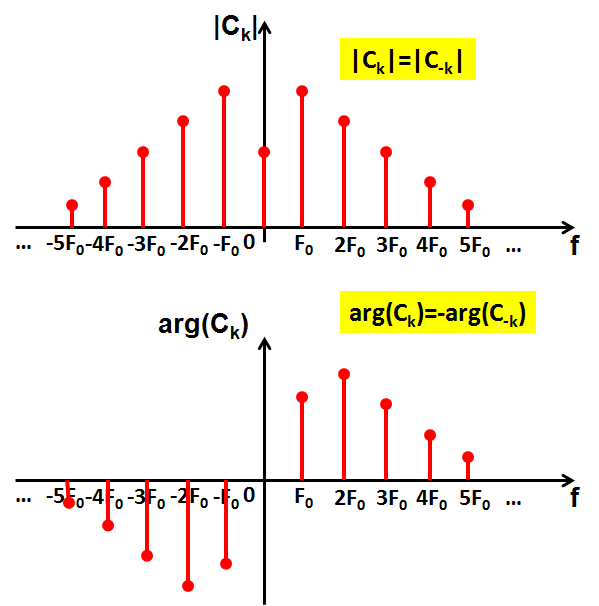
\includegraphics[scale=0.5]{images/Exemple_spectre.png}
		\caption{Exemple de représentation du spectre de raies en amplitude (en haut) et en phase (en bas)}	
		\label{Fig:Spectre_raies} 
	\end{figure}
	 

	
	\subsection{Analyse spectrale d'un signal}
	
	Le développement en série de Fourier permet l'analyse spectrale d'un signal périodique, c'est-à-dire la richesse en composantes harmoniques. L'analyse du signal dans le domaine temporel ne le permet pas nécessairement.
	
	Lorsqu'un signal ne contient qu'une composante fondamentale, on parle de signal monochromatique. Par exemple, le signal sonore généré par un diapason, est caractérisé par une fréquence fondamentale égale à 44 0Hz. Ce type de signal est modélisé par une
	fonction exponentielle de la forme $Re[e^{j\omega_{0}t}]$ où $\omega_{0}=2\pi x440$. Pour un instrument de musique, cette fréquence fondamentale est accompagnée de fréquences 	harmoniques c'est-à-dire de composantes sonores dont les fréquences sont des multiples de la fréquence fondamentale. La richesse en harmoniques donne à l'instrument sa spécificité et son timbre pour chaque note. Si on s'intéresse maintenant au langage parlé, les voyelles sont des sons composés de la superposition de signaux dont les fréquences sont des multiples entiers 	d'une fréquence fondamentale appelée hauteur du son (\textit{pitch} en anglais). Le phénomène physique
	de génération du son d'une voyelle repose sur l'impact des cordes vocales qui obturent
	périodiquement l'écoulement continu de l'air provenant des poumons. En aval des cordes, on pourrait mesurer une succession d'impulsions de pression d'air. La fréquence fondamentale de	ces impulsions est d'environ 100 Hz pour les hommes et 200 Hz pour les femmes. Ces impulsions répétitives très brèves sont riches en harmoniques. Le son d'une voyelle différera de celui d'une autre voyelle par l'importance respective des différentes harmoniques.\\



	
	\section{Excitation d'un système linéaire par un signal périodique}
	Lorsqu'un signal périodique x(t) excite un système linéaire à temps invariant, sa réponse peut être facilement déterminée à partir de la décomposition en série de Fourier de l'excitation. C'est ce qu'illustre la figure \ref{Fig:Excitation d'un système linéaire par un signal périodique}. En effet, en raison des propriétés de linéarité du développement en série de Fourier, la réponse y(t) sera égale à la décomposition en série de Fourier de l'excitation x(t), mais dont les coefficients $C_k$ seront pondérés par la fonction de transfert du système H en chacune des fréquences harmoniques de l'excitation. Cette propriété offre un moyen alternatif à la transformée de Laplace pour calculer la réponse d'un système linéaire.
	\begin{equation}\label{key}
	y(t)=\sum_{k=-\infty}^{+\infty}H(k\omega_{0})C_ke^{jk\omega_{0}}
	\end{equation}
	 
	 \begin{figure}[h!]
	 	\centering
	 	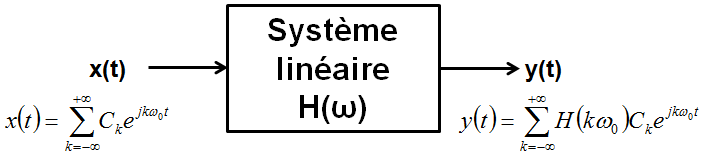
\includegraphics[scale=0.6]{images/LTI_serie_Fourier.png}
	 	\caption{Exemple de représentation du spectre de raies en amplitude (en haut) et en phase (en bas)}	
	 	\label{Fig:Excitation d'un système linéaire par un signal périodique} 
	 \end{figure}
	 
	Une autre propriété des systèmes linéaires apparait ici : lorsqu'il est excité par un signal avec un contenu spectral donné, un système linéaire ne peut enrichir ce contenu spectrale. Autrement dit, de nouvelles composantes harmoniques ne peuvent pas apparaitre si le système est linéaire. Autrement, le système est non-linéaire.
	 
	 
	 
	
	\section{Egalité de Parseval}
	
	On considère un signal périodique x(t) de période $T_{0}$, décomposable  une série de Fourier. Chaque terme de la série de Fourier contribue à une partie de la puissance du signal. La puissance moyenne $P_{n}$ de chacun de ces membres peut être reliée au coefficient de Fourier, dans leur version complexe selon \ref{Parseval_complexe}. Chacun des coefficients au carré est homogène à une puissance.
	\begin{equation}\label{Parseval_complexe}
	P_{n}=\frac{1}{T_{0}}\int_{T_{0}}|x(t)|^{2}dt=\sum_{k=-\infty}^{+\infty}|C_k|^{2}
	\end{equation}
	La même égalité peut s'écrire avec la version trigonométrique : 
	\begin{equation}\label{Parseval_trigo}
	P_{n}=\frac{1}{T_{0}}\int_{T_{0}}|x(t)|^{2}dt=|A_0|^{2}+\frac{1}{2}\sum_{k=1}^{+\infty}(|A_k|^{2}+|B_k|^{2})
	\end{equation}

	
	Nous reviendrons sur les questions de puissance et d'énergie des signaux au chapitre 8.\\
	
	
	\section{Exercices}
	
\subsubsection{Exercice 1}
	Développez en série de Fourier la fonction $f(t)=|sin(\alpha t)|$ avec $\alpha \in \mathbb{R^{*}}$ donné.\\
	
	\subsubsection{Exercice 2}
	Soit f : $\mathbb{R} \rightarrow \mathbb{R}$ une fonction périodique de période 4, impaire, définie par :
	\begin{equation*}
	f(t)=\left \{
	\begin{array}{l}
	1-t~~si~t~\in[0;1[ \\
	0~~si~t~\in[1;2[ \\
	\end{array}
	\right .
	\end{equation*}
	
	1. Dessinez le graphe de f. Calculer f(7), f($\frac{9}{2})$ et $f(\frac{11}{2})$.\\
	
	2. Calculez les coefficients de Fourier de f.\\
	
	\subsubsection{Exercice 3}
	Cet exercice est en relation avec l'exemple d'un signal rectangulaire présenté dans le cours. On considère un signal de même nature, de moyenne nulle, de période $T_1$, de fréquence $f_1$ et	d'amplitude 2, représenté par la fonction périodique s. On s'intéresse au produit scalaire de la fonction s avec les fonctions de base $cos(n\omega_{1}t)$, n = 1, 2 et 3 où $\omega_{1} = \frac{2\pi}{T_1}$. La figure ci-dessous représente sur la première ligne, dans la colonne de gauche, le graphe de la fonction s superposé à celui de	la fonction $cos(\omega_{1}t)$ et dans la colonne de droite, le graphe du produit scalaire $s(t)cos(\omega_{1}t)$ sur
	une période $T_1$. Sur la deuxième ligne sont représentés, dans la colonne de gauche, le graphe de la fonction s superposé à celui de la fonction $cos(2\omega_{1}t)$ et dans la colonne de droite, le graphe	du produit scalaire $s(t)cos(2\omega_{1}t)$ sur une période $T_1$. Sur la troisième ligne sont représentés,
	dans la colonne de gauche, le graphe de la fonction s superposé à celui de la fonction  $cos(3\omega_{1}t)$	et dans la colonne de droite, le graphe du produit scalaire $s(t)cos(3\omega_{1}t)$ sur une période $T_1$. 
	
	\begin{figure}[h!]
		\centering
		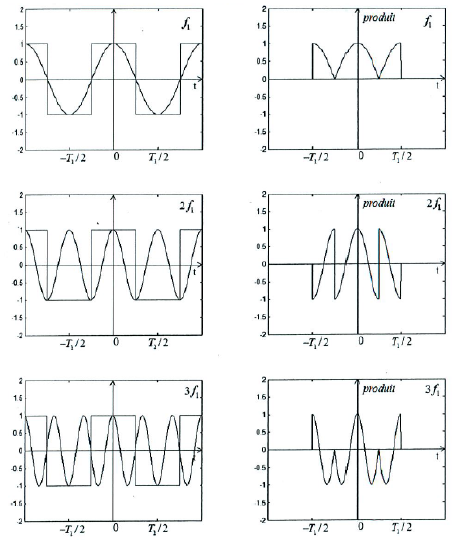
\includegraphics[scale=0.8]{images/Exo_Fourier_Lea.png}
		\caption{Colonne de gauche : graphe de s et de $cos(\omega_{1}t)$, $cos(2\omega_{1}t)$, $cos(3\omega_{1}t)$ - Colonne de droite
			: graphes de $s(t)cos(\omega_{1}t)$, $s(t)cos(2\omega_{1}t)$ et $s(t)cos(3\omega_{1}t)$.}	
		\label{Fig:Exo_Fourier_signal_carré} 
	\end{figure}

	1. Définir la fonction s.\\
	2. Que représente le produit scalaire de s par une fonction de base $cos(n\omega_{1}t)$, n = 1, 2 ou 3 ?\\
	3. Interpréter qualitativement (sans calcul) les trois produits scalaires représentés sur la figure \ref{Fig:Exo_Fourier_signal_carré} en donnant leur signe et une indication de leur valeur algébrique.\\
	4. A quel résultat (sans calcul) peut-on s'attendre si on effectue le produit scalaire de s par les fonctions de bases $sin(n\omega_{1}t)$, n = 1, 2 ou 3 ? ?\\
	5. En considérant le signal s comme un signal retardé par rapport au signal étudié en
	cours et en utilisant les résultats établis dans le cours, calculer les coefficients de Fourier exponentiels de s. Donner la série de Fourier associée à s.\\
	
	
	\subsubsection{Exercice 4}
	Soit f une fonction définie sur l'intervalle [0;1] de $\mathbb{R}$ par f(t) = t.
	On considère f comme la restriction de fonctions $g_i$ avec i = 1, 23 3, périodiques et continues par morceaux sur $\mathbb{R}$. On se propose de déterminer plusieurs expressions de f sur ]0;1[ à partir du développement en séries de Fourier des fonctions $g_i$.\\
	
	1. On considère la fonction $g_1$, périodique, de période $T_1$ = 3, définie par $\forall t \in [0;3[~~ g_1(t) = t$.\\
		a. Représentez la fonction $g_1$ sur l'intervalle [-3;6].
		
		b. Calculez les coefficients de Fourier de $g_1$ et donnes la série de Fourier $S_1$ associée à $g_1$.
		
		
		c. Etudiez la convergence de $S_1$.
		
		d. En déduire le développement en série de Fourier de f sur ]0;1[.\\
		
	2. On considère la fonction $g_2$, impaire, périodique, de période $T_2$ = 2, définie par $\forall t \in [0;1[~~ g_2(t) = t$.\\
		a. Représentez la fonction $g_2$ sur l'intervalle [-3;3].
		
		b. Calculez les coefficients de Fourier de $g_2$ et donnes la série de Fourier $S_2$ associée à $g_2$.
		
		c. Etudiez la convergence de $S_2$.
		
		d. En déduire le développement en série de Fourier de f sur ]0;1[.\\
	
	3. On considère la fonction $g_3$, paire, périodique, de période $T_3$ = 2, définie par $\forall t \in [0;1[~~ g_3(t) = t$.\\
		a. Représentez la fonction $g_3$ sur l'intervalle [-4;4].
	
		b. Calculez les coefficients de Fourier de $g_3$ et donnes la série de Fourier $S_3$ associée à $g_3$.
	
		c. Etudiez la convergence de $S_3$.
	
		d. En déduire le développement en série de Fourier de f sur ]0;1[.\\
	
	
	\subsubsection{Exercice 5}
	
	Donnez la définition, la période et la parité des fonctions représentées par les séries de Fourier suivantes et tracez leur graphe :\\
	
	1. $	\frac{2}{\pi}-\frac{4}{\pi}\sum_{n=1}^{+\infty}cos(2nt)=sin(t)~~avec~t~\in[0;\pi]$\\
	
	2. $	2\sum_{n=1}^{+\infty}\frac{1-(-1)^{n}}{n \pi}sin(n \pi t)=1~~avec~t~\in[0;1]$ \\
	
	3. $	\pi-\sum_{n=1}^{+\infty}\frac{2}{n}sin(nt)=t~~avec~t~\in[0;2\pi]$ \\
	
	
	\subsubsection{Exercice 6 - Signal de forme exponentielle}
	On considère la fonction x définie sur $\mathbb{R}$ à valeurs dans $\mathbb{R}$, de période $T=2\pi$, par $x(t)=e^{t}$ pour $t\in [0;+2\pi[$.\\
	
	1. Tracez la fonction x(t) sur l'intervalle $[-2\pi;+2\pi[$.\\
	
	2. Cette fonction admet-elle un développement en série de Fourier ?\\
	
	3. Montrez que les coefficients de Fourier sous la forme exponentielle sont égaux à $c_{n}=\frac{1+jn}{2\pi(1+n^{2})}(e^{2\pi}-1)~~\forall n \in \mathbb{Z}$.\\
	
	4. En déduire les expressions des coefficients de Fourier sous leur forme trigonométriqque.\\
	
	5. Calculez la puissance moyenne des harmoniques, quelle que soit leur rang.\\
	
	6. Calculez la puissance moyenne du signal.\\
	

	
	
	\subsubsection{Exercice 7 - Modulation à largeur d'impulsion}
	La modulation à largeur d'impulsion (MLI) (Pulse Width Modulation PWM en anglais) est une technique couramment utilisée en électronique pour générer un signal analogique à partir d'un signal discret à deux états. Le signal MLI $s_p(t)$ est constitué d'une suite périodique, de période T, d'impulsions $s_i(t)$ définie par :
	\begin{equation*}
	s_i(t)=\left \{
	\begin{array}{l}
	A~~si~t~\in[0;\alpha T] \\
	0~~sinon \\
	\end{array}
	\right .
	\end{equation*}   
	où $\alpha \in [0;1]$ est appelé le rapport cyclique du signal (duty ratio en anglais). Le principe est illustré à la figure \ref{Fig:signal_MLI}. A partir d'un signal analogique de valeurs comprises entre 0 et A, un modulateur MLI va produire le signal MLI à partir de deux niveaux de tension seulement.\\
	
	\begin{figure}[h!]
		\centering
		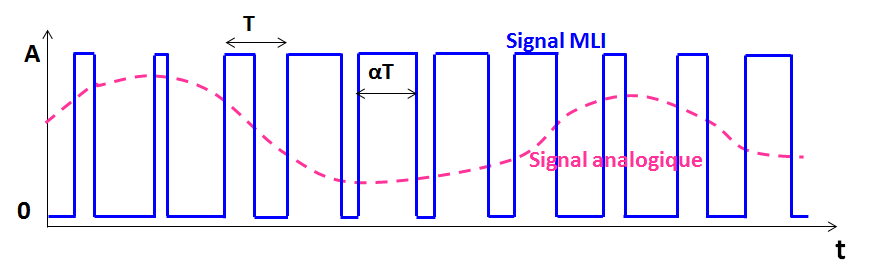
\includegraphics[scale=0.6]{images/signal_MLI.png}
		\caption{Illustration modulation MLI}	
		\label{Fig:signal_MLI} 
	\end{figure}
	
	1. Vérifiez si on peut développer $s_i(t)$ et $s_p(t)$ en séries de Fourier. \\
	
	2. Calculez les coefficients de Fourier exponentiels du signal MLI $s_p(t)$ et vérifiez la relation avec les coefficients de Fourier réels.\\
	
	3. Que deviennent ces coefficients si l'on considère le signal $s_p(t)$ de même période mais retardé d'un temps $\tau \in \mathbb{R^{*}}$.\\
	
	4. Calculez la puissance moyenne du signal, ainsi que celles de la somme de tous les termes de la série de Fourier. Sont-elles égales ?\\
	
	5. Quelle est la puissance moyenne transportée par le premier harmonique ?\\
	
	6. Une manière économique de reconstituer un signal analogique à partir du signal MLI est de le filtrer, à l'aide d'un filtre passe-bas que l'on supposera idéal. Sa fréquence de coupure est notée $f_c$. Quelle est la forme du signal selon $f_c$ ? Quelle fréquence de coupure choisiriez-vous pour que le signal en sortie du filtre soit constant et proportionnel au rapport cyclique ? Est-ce un bon choix pour reconstituer le signal analogique ?\\
	
	7. Quelle est l'énergie du signal en sortie du filtre ? En déduire le rendement du système de conversion ?\\
	


	
	
	